\section{The critical scaling function}
\label{sec:critical-scaling}

The transition scale $\beta\asymp n^{-2}$ admits a limiting spectral
problem with an explicit finite-size error.  We write $\gamma_Q(n,\beta)$
for the gap of the count chain with birth rates $\beta(n-k)$ and death
rates $k(k-1)/n$.  By Theorem~\ref{thm:exact-gap}, it equals the polymer
gap $\gamma_M(n,\beta)$.

For $b>0$, define a killed birth--death operator on the positive integers
by
\begin{equation}\label{eq:critical-infinite-operator}
 (\mathcal A_b f)(k)
 =b[f(k+1)-f(k)]+k(k-1)[f(k-1)-f(k)]-2kf(k),
 \qquad k\geq1.
\end{equation}
The backward term at $k=1$ is zero.  Its underlying conservative chain
has reversible probability measure
\begin{equation}\label{eq:critical-weight}
 \pi_b(k)=Z_b^{-1}\frac{b^{k-1}}{k!(k-1)!},
 \qquad
 Z_b=\sum_{k\geq1}\frac{b^{k-1}}{k!(k-1)!}.
\end{equation}
All moments of $\pi_b$ are finite.

\begin{proposition}[Construction of the limiting operator]
\label{prop:critical-operator}
On $\ell^2(\pi_b)$, the quadratic form
\begin{equation}\label{eq:critical-form}
 \mathcal E_b(f,f)
 =\sum_{k\geq1}\pi_b(k)b[f(k+1)-f(k)]^2
   +\sum_{k\geq1}2k\pi_b(k)f(k)^2
\end{equation}
with domain consisting of the functions for which this expression is
finite is densely defined and closed.  Its associated self-adjoint
operator $H_b=-\mathcal A_b$ has compact resolvent.  Its smallest
eigenvalue $\rho(b)$ is simple and has a strictly positive eigenfunction
$h_b$.
\end{proposition}

\begin{proof}
Detailed balance follows from
$\pi_b(k)b=\pi_b(k+1)k(k+1)$.  Closedness of the form follows by taking
coordinate limits of a Cauchy sequence in the form norm and using the
nonnegative sums in~\eqref{eq:critical-form}.  Finitely supported
functions form a core.  Indeed, for $f$ in the form domain, truncate it
at $R$.  The only extra edge term in the squared form norm of the
discarded tail is $\pi_b(R)b f(R+1)^2$, and
\[
 \pi_b(R)b f(R+1)^2
 \leq 2\pi_b(R)b[f(R+1)-f(R)]^2
       +2\pi_b(R)b f(R)^2\longrightarrow0.
\]
All the other terms are tails of convergent nonnegative series.

The form domain is compactly embedded in $\ell^2(\pi_b)$: for every
$R\geq1$,
\begin{equation}\label{eq:critical-compact-tail}
 \sum_{k>R}\pi_b(k)f(k)^2
 \leq\frac{\mathcal E_b(f,f)}{2(R+1)}.
\end{equation}
Thus a bounded set in the form norm has uniformly small tails, while
each finite-coordinate projection is precompact.  The associated
operator therefore has compact resolvent, and the bottom of its
spectrum is attained.  Taking the absolute value does not increase the
form.  A nonnegative eigenfunction at the bottom is strictly positive:
the coordinate eigenvalue equation propagates any zero to both
neighbors, and hence to every state.  Finally, the equation at $k=1$
determines $h(2)$ from $h(1)$; the subsequent three-term recurrence
determines all remaining coordinates.  The lowest eigenspace is
therefore one-dimensional.
\end{proof}

The next ratio estimate will control both the limit and its finite
approximations.  The finite count-derivative operator is
\begin{equation}\label{eq:critical-finite-derivative}
 \begin{split}
 (A_{n,\beta}h)(k)
 ={}&\beta(n-k-1)[h(k+1)-h(k)]\\
 &+\frac{k(k-1)}n[h(k-1)-h(k)]
   -\left(\beta+\frac{2k}n\right)h(k),
 \qquad 1\leq k\leq n-1.
 \end{split}
\end{equation}
Its spectrum is the nonzero spectrum of the count generator, with the
same signs.

\begin{lemma}[Ground-state ratios]
\label{lem:critical-ground-ratios}
Let $h$ be a positive ground state of either $-A_{n,\beta}$ or $H_b$.
At every pair of successive states in its domain,
\begin{equation}\label{eq:critical-ratio-bounds}
 \frac{k+1}{k+3}\leq\frac{h(k+1)}{h(k)}\leq1.
\end{equation}
In particular, $h_b$ is bounded.
\end{lemma}

\begin{proof}
A nonexplosive birth--death chain on an interval has an order-preserving
coupling.  Run two copies independently until they meet and then
coalesce them.  Nearest-neighbor paths cannot cross without meeting.
Consequently the Feynman--Kac survival function
\[
 k\longmapsto
 \mathbb E_k\exp\left\{-\int_0^t V(X_s)\,ds\right\}
\]
is decreasing when the killing potential $V$ is increasing, and is
increasing when $V$ is decreasing.  The conservative chain underlying
$\mathcal A_b$ is nonexplosive: its births have constant rate $b$, and
the number of deaths by any time is at most the initial population
minus one plus the number of births.  All finite chains here are
nonexplosive as well.

For the original killed operators the potentials are $\beta+2k/n$ and
$2k$, respectively, and hence are increasing.  Their survival functions
are decreasing in $k$.  The spectral projection onto the simple
positive ground state, after multiplication by the exponential of the
lowest eigenvalue, converges in the reversible $\ell^2$ space and
therefore at each coordinate.  Applied to the constant function, this
shows that $h$ is decreasing.

For the other inequality set
\[
 h_0(k)=\frac1{(k+1)(k+2)}.
\]
Conjugating the killed operator by multiplication by $h_0$ gives a
birth--death operator whose new killing potential is, respectively,
\begin{equation}\label{eq:critical-transform-potentials}
 \begin{split}
 -\frac{A_{n,\beta}h_0(k)}{h_0(k)}
 &=\beta+\frac2n+\frac{2\beta(n-k-1)}{k+3}
   =\frac2n-\beta+\frac{2\beta(n+2)}{k+3},\\
 -\frac{\mathcal A_bh_0(k)}{h_0(k)}
 &=2+\frac{2b}{k+3}.
 \end{split}
\end{equation}
Both are positive and decreasing.  The transformed birth and death
rates in the infinite case are
\[
 b\frac{k+1}{k+3},\qquad (k-1)(k+2).
\]
Its birth rates are bounded by $b$, so the same argument proves
nonexplosion.  The transformed reversible measure is proportional to
$\pi_b h_0^2$, and multiplication by $h_0$ is a unitary identification
with the original weighted space, up to an irrelevant normalization.
The transformed ground state is $h/h_0$.  Applying the preceding
survival-function argument to the decreasing potential shows that
$h/h_0$ is increasing.  Since
$h_0(k+1)/h_0(k)=(k+1)/(k+3)$, this proves the lower ratio bound.

For completeness, in the infinite case the Feynman--Kac semigroups
used here are the semigroups of the form operators.  One may first kill
the conservative paths upon leaving a finite interval and then let
that interval increase.  Nonexplosion gives the pathwise limit, and
the finitely supported form core established above identifies its
operator with $H_b$.  The same argument applies after conjugation by
$h_0$.  Thus the spectral projection and the order comparison concern
the same semigroup.
\end{proof}

\begin{theorem}[Critical limit with a finite-size error]
\label{thm:critical-limit}
For all $n\geq2$ and $b>0$,
\begin{equation}\label{eq:critical-finite-error}
 \left|n\gamma_M\left(n,\frac b{n^2}\right)-\rho(b)\right|
 \leq\frac bn.
\end{equation}
The same statement holds with $\gamma_Q$ in place of $\gamma_M$.
\end{theorem}

\begin{proof}
Restrict $h_b$ to $1,\ldots,n-1$.  The infinite eigenvalue equation
gives the exact identity
\begin{equation}\label{eq:critical-finite-quotient}
 -\frac{nA_{n,b/n^2}h_b(k)}{h_b(k)}
 =\rho(b)+\frac bn
   \left[1+(k+1)\left(\frac{h_b(k+1)}{h_b(k)}-1\right)\right].
\end{equation}
This includes the upper endpoint $k=n-1$: the finite birth rate there
is zero, and the displayed correction accounts for removal of the
infinite birth term.  By~\eqref{eq:critical-ratio-bounds}, the bracket
lies between $-1+4/(k+3)$ and $1$, and hence between $-1$ and $1$.
Positive-vector comparison for the finite killed chain proves the
claim for $\gamma_Q$.  Theorem~\ref{thm:exact-gap} then gives the claim
for $\gamma_M$.
\end{proof}

\begin{proposition}[Continuity and moving critical parameters]
\label{prop:critical-lipschitz}
For $0<b_1\leq b_2$,
\begin{equation}\label{eq:critical-lipschitz}
 0\leq\rho(b_2)-\rho(b_1)\leq\frac{b_2-b_1}{2}.
\end{equation}
Moreover,
\begin{equation}\label{eq:critical-elementary-bounds}
 2<\rho(b)\leq2+\frac b2\qquad(b>0).
\end{equation}
Thus $\rho$ extends continuously to $b=0$ by $\rho(0)=2$.  If
$\beta_n>0$ and $b_n=n^2\beta_n\longrightarrow b\in[0,\infty)$, then
\begin{equation}\label{eq:critical-moving-parameter}
 \left|n\gamma_M(n,\beta_n)-\rho(b)\right|
 \leq\frac{b_n}{n}+\frac{|b_n-b|}{2}\longrightarrow0.
\end{equation}
\end{proposition}

\begin{proof}
Write $h_i=h_{b_i}$ and $\delta=b_2-b_1$.  Pointwise,
\[
 H_{b_2}h_1
 =\rho(b_1)h_1+\delta[h_1(k)-h_1(k+1)].
\]
The ratio lemma implies
\begin{equation}\label{eq:critical-parameter-quotient}
 0\leq\frac{h_1(k)-h_1(k+1)}{h_1(k)}
 \leq\frac2{k+3}\leq\frac12.
\end{equation}
This identity may legitimately be paired with $h_2$ in
$\ell^2(\pi_{b_2})$.  Indeed, $h_1$ is bounded; the weight
$\pi_{b_2}$ has all moments, so $h_1$ is in the form domain of
$H_{b_2}$.  The displayed pointwise expression for $H_{b_2}h_1$ is
bounded and hence square integrable.  Summation by parts against
finitely supported test functions, followed by the form-core
approximation, puts $h_1$ in the operator domain.  Self-adjointness
therefore yields
\[
 [\rho(b_2)-\rho(b_1)]\langle h_2,h_1\rangle_{\pi_{b_2}}
 =\delta\langle h_2,h_1-h_1(\cdot+1)\rangle_{\pi_{b_2}}.
\]
The inner product on the left is strictly positive.  Dividing and
using~\eqref{eq:critical-parameter-quotient} proves
\eqref{eq:critical-lipschitz}.

The potential term in~\eqref{eq:critical-form} gives $\rho(b)\geq2$;
strict positivity of the ground state at states $k>1$ makes the
inequality strict.  At $k=1$ the eigenvalue equation reads
\[
 \rho(b)=2+b\left(1-\frac{h_b(2)}{h_b(1)}\right)\leq2+\frac b2.
\]
This proves the extension at zero.  Finally,
\eqref{eq:critical-moving-parameter} follows from
Theorem~\ref{thm:critical-limit} and the Lipschitz estimate.
\end{proof}

\begin{proposition}[Finite-matrix brackets]
\label{prop:critical-truncation}
For an integer $R\geq1$, suppress the birth at $R$ in
\eqref{eq:critical-infinite-operator} and retain the same killing
$2k$ on $1,\ldots,R$.  Let $\rho_R(b)$ be the smallest eigenvalue of
the negative of this finite killed generator.  Then
\begin{equation}\label{eq:critical-truncation-error}
 \rho_R(b)\leq\rho(b)
 \leq\rho_R(b)+\frac{2b}{R+3}.
\end{equation}
Equivalently, $\rho_R(b)$ is the smallest eigenvalue of the symmetric
tridiagonal matrix $J_R(b)$ with entries
\begin{equation}\label{eq:critical-jacobi-matrix}
 \begin{split}
 (J_R)_{kk}&=k(k+1)+b\,\mathbf1_{\{k<R\}},\qquad 1\leq k\leq R,\\
 (J_R)_{k,k+1}&=(J_R)_{k+1,k}=-\sqrt{bk(k+1)},
       \qquad 1\leq k<R.
 \end{split}
\end{equation}
\end{proposition}

\begin{proof}
Restrict $h_b$ to $1,\ldots,R$.  Its positive-vector quotient is
$\rho(b)$ at all states below $R$, while at $R$ it is
\[
 \rho(b)-b\left(1-\frac{h_b(R+1)}{h_b(R)}\right)
 \in\left[\rho(b)-\frac{2b}{R+3},\rho(b)\right].
\]
Finite positive-vector comparison proves
\eqref{eq:critical-truncation-error}, including $R=1$.  Conjugation by
the square root of the finite reversible weights gives
\eqref{eq:critical-jacobi-matrix}.
\end{proof}

The brackets above give an explicit approximation of the critical
scaling function without an unquantified infinite-state truncation.
If a finite-matrix computation supplies rigorous bounds
$a_R\leq\rho_R(b)\leq c_R$, then
$[a_R,c_R+2b/(R+3)]$ is a rigorous interval for $\rho(b)$.

\subsection{The degree-one critical scaling function}

The degree-one eigenvalue in the spatial theorem has a parallel
limit.  On the nonnegative integers define
\begin{equation}\label{eq:critical-degree-one-operator}
 (\mathcal A_b^{(1)}f)(j)
 =b[f(j+1)-f(j)]+j^2[f(j-1)-f(j)]-jf(j),
 \qquad j\geq0.
\end{equation}
Its reversible weights are
\[
 \nu_b(j)=\widehat Z_b^{-1}\frac{b^j}{(j!)^2}.
\]
Use the closed form
\[
 \mathcal F_b(f,f)
 =\sum_{j\geq0}\nu_b(j)b[f(j+1)-f(j)]^2
   +\sum_{j\geq0}j\nu_b(j)f(j)^2
\]
to define $H_b^{(1)}=-\mathcal A_b^{(1)}$.  The form-core and
compactness arguments of Proposition~\ref{prop:critical-operator}
apply verbatim, with the tail bound
$\sum_{j>R}\nu_b(j)f(j)^2\leq\mathcal F_b(f,f)/(R+1)$.
Thus $H_b^{(1)}$ has a simple positive ground state $g_b$ and a
smallest eigenvalue $\sigma(b)>0$.  Positivity of this eigenvalue
follows because zero form energy would force a constant function
vanishing at every $j\geq1$.

\begin{proposition}[Degree-one critical approximation]
\label{prop:critical-degree-one}
For all $n\geq2$ and $b>0$,
\begin{equation}\label{eq:critical-degree-one-error}
 0\leq n\eta_1\left(n,\frac b{n^2}\right)-\sigma(b)
 \leq\frac bn.
\end{equation}
The limiting eigenvalue satisfies
\begin{equation}\label{eq:critical-degree-one-bounds}
 \frac{b}{\sqrt b+2}\leq\sigma(b)
 \leq\min\left\{\sqrt b,\frac b2\right\}.
\end{equation}
It is increasing and $1/2$-Lipschitz, and extends continuously to zero
by $\sigma(0)=0$.
\end{proposition}

\begin{proof}
The killing $j$ is increasing, so the order-preserving survival
comparison used in Lemma~\ref{lem:critical-ground-ratios} makes $g_b$
decreasing.  Conjugation by $g_0(j)=1/(j+1)$ yields the decreasing
killing potential $b/(j+2)$ and birth and death rates
$b(j+1)/(j+2)$ and $j(j+1)$.  Its births are bounded and its chain
is nonexplosive.  The same transformed-semigroup argument gives
\begin{equation}\label{eq:critical-degree-one-ratios}
 \frac{j+1}{j+2}\leq\frac{g_b(j+1)}{g_b(j)}\leq1.
\end{equation}

Set $j=k-1$ in the finite operator~\eqref{eq:spatial-degree-one}
and test it with $g_b$.  Its exact quotient is
\[
 -\frac{nA_1g_b(j)}{g_b(j)}
 =\sigma(b)+\frac bn
   \left[1+(j+2)\left(\frac{g_b(j+1)}{g_b(j)}-1\right)\right],
 \qquad 0\leq j\leq n-2,
\]
where $A_1$ here is expressed in the shifted coordinate.
The bracket belongs to $[0,1]$, including the upper endpoint where
the finite birth rate vanishes.  Positive-vector comparison proves
\eqref{eq:critical-degree-one-error}.

For the bounds put $a=\sqrt b$ and test the infinite operator with
$f(j)=1/(j+1+a)$.  Its quotient is
\[
 -\frac{\mathcal A_b^{(1)}f(j)}{f(j)}
 =a-\frac{2a^2}{(j+a)(j+a+2)}
 \in\left[\frac{a^2}{a+2},a\right].
\]
This test function is bounded and belongs to the operator domain;
pairing its equation with the positive ground state justifies the
infinite-state comparison, exactly as in the proof of
Proposition~\ref{prop:critical-lipschitz}.  The equation at $j=0$
also gives
$\sigma(b)=b[1-g_b(1)/g_b(0)]\leq b/2$.
Finally, changing $b_1$ to $b_2\geq b_1$ adds
$(b_2-b_1)[1-g_{b_1}(j+1)/g_{b_1}(j)]$ to the quotient.  This lies
in $[0,(b_2-b_1)/2]$ by
\eqref{eq:critical-degree-one-ratios}.  The cross-parameter domain
argument and positive-ground-state pairing in
Proposition~\ref{prop:critical-lipschitz} apply with $\nu_b$ in
place of $\pi_b$.  They prove the stated monotonicity and Lipschitz
bound; the estimate $\sigma(b)\leq b/2$ supplies continuity at zero.
\end{proof}

\begin{corollary}[The ends of the crossover]
\label{cor:critical-end-asymptotics}
The limiting functions satisfy
\begin{equation}\label{eq:critical-end-asymptotics}
 \begin{aligned}
 &\rho(b)\longrightarrow2,\qquad
   \sigma(b)\sim b/2 &&\text{as }b\downarrow0,\\
 &\rho(b)\sim2\sqrt b,\qquad
   \sigma(b)\sim\sqrt b &&\text{as }b\longrightarrow\infty.
 \end{aligned}
\end{equation}
In particular, the count and spatial degree-one modes have different
leading constants at the large-$b$ end of the critical scaling.
\end{corollary}

\begin{proof}
The assertions for $\sigma$ follow by squeezing with
\eqref{eq:critical-degree-one-bounds}; the limit of $\rho$ at zero
was proved in Proposition~\ref{prop:critical-lipschitz}.
For fixed $b>0$, apply the additive-error estimate of
Theorem~\ref{thm:sharp-gap} at $\beta=b/n^2$, multiply by $n$, and
then let $n\to\infty$ using Theorem~\ref{thm:critical-limit}.
This gives
\[
 2\sqrt b-5\leq\rho(b)\leq2\sqrt b+4,
\]
which proves the last asymptotic equivalent.
\end{proof}

For numerical approximation of $\sigma$, suppress the birth at an
integer $R\ge0$ and retain the killing $j$ on $0,\ldots,R$.
Let $\sigma_R(b)$ be the lowest eigenvalue of this finite operator.
The same restricted-ground-state argument as in
Proposition~\ref{prop:critical-truncation}, now using
\eqref{eq:critical-degree-one-ratios}, gives
\begin{equation}\label{eq:critical-sigma-truncation}
 0\le\sigma(b)-\sigma_R(b)\le\frac{b}{R+2}.
\end{equation}
Indeed, only the last quotient changes, by
$-b[1-g_b(R+1)/g_b(R)]$. The corresponding symmetric matrix has
diagonal $j(j+1)+b\mathbf1_{\{j<R\}}$ and off-diagonal
$-\sqrt b(j+1)$ between $j$ and $j+1$.

\begin{corollary}[The joint critical spatial limit]
\label{cor:critical-spatial-limit}
For every $n\geq2$, $b>0$, connected weighted graph $G$ on $n$
vertices and $D\geq0$,
\begin{equation}\label{eq:critical-spatial-error}
 \left|n\gamma_{\mathrm{sp}}\left(n,\frac b{n^2},D,G\right)
 -\min\{\rho(b),\sigma(b)+nD\lambda_G\}\right|
 \leq\frac bn.
\end{equation}
Consequently, if $n^2\beta_n\to b\in[0,\infty)$ and
$nD_n\lambda_{G_n}\to\delta\in[0,\infty)$, then
\begin{equation}\label{eq:critical-spatial-limit}
 n\gamma_{\mathrm{sp}}(n,\beta_n,D_n,G_n)
 \longrightarrow\min\{\rho(b),\sigma(b)+\delta\}.
\end{equation}
If instead $nD_n\lambda_{G_n}\to\infty$, the limit is $\rho(b)$.
\end{corollary}

\begin{proof}
Apply Theorem~\ref{thm:spatial-exact-gap},
Theorem~\ref{thm:critical-limit}, and
Proposition~\ref{prop:critical-degree-one}.  The minimum of two
real numbers is $1$-Lipschitz for their maximum-coordinate distance.
For moving parameters use the continuity of $\rho$ and $\sigma$.
\end{proof}

Figure~\ref{fig:scaling-limits} illustrates the inverse-mass limit
and the two critical scaling functions.
\begin{figure}[htbp]
 \centering
 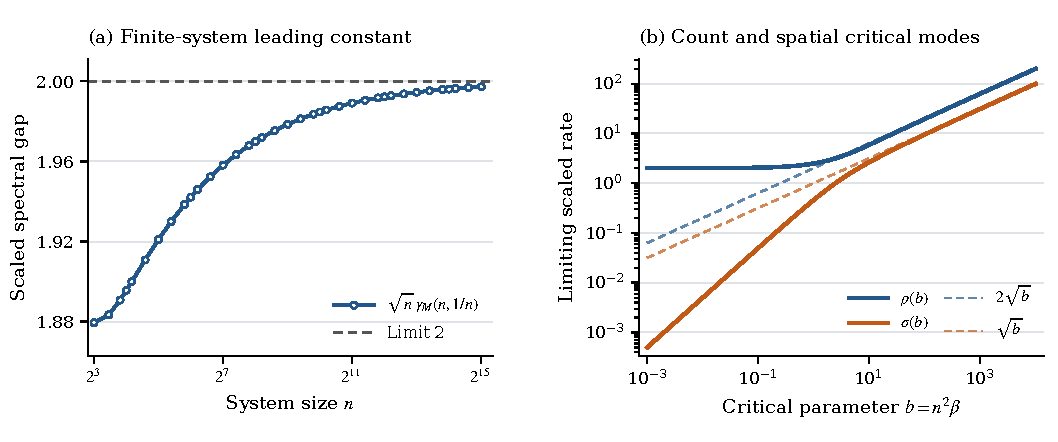
\includegraphics[width=\linewidth]{scaling_limits.pdf}
 \caption{Spectral scaling from finite radial matrices.
 (a) Direct numerical eigenvalues of the count derivative give
 $\sqrt n\,\gamma_M(n,1/n)$ approaching $2$.
 (b) Finite Jacobi approximations to $\rho(b)$ and $\sigma(b)$,
 with their large-$b$ equivalents $2\sqrt b$ and $\sqrt b$.
 The faint bands show the analytic truncation widths
 $2b/(R+3)$ and $b/(R+2)$, respectively, where
 $R=\lceil600(1+\sqrt b)\rceil$.
 Finite eigenvalues are evaluated in floating point; the bands do
 not include a certified rounding-error interval.
 Source data and the plotting program accompany the paper.}
 \label{fig:scaling-limits}
\end{figure}
